\section{Development Environment}\label{section:development-environment3}

This section presents the web-based development environment, which is the part of \tool that learners are interacting with during their programming session. Figure~\ref{figure:development-environment1} depicts the application from a learner's perspective.

\begin{figure}
\centering
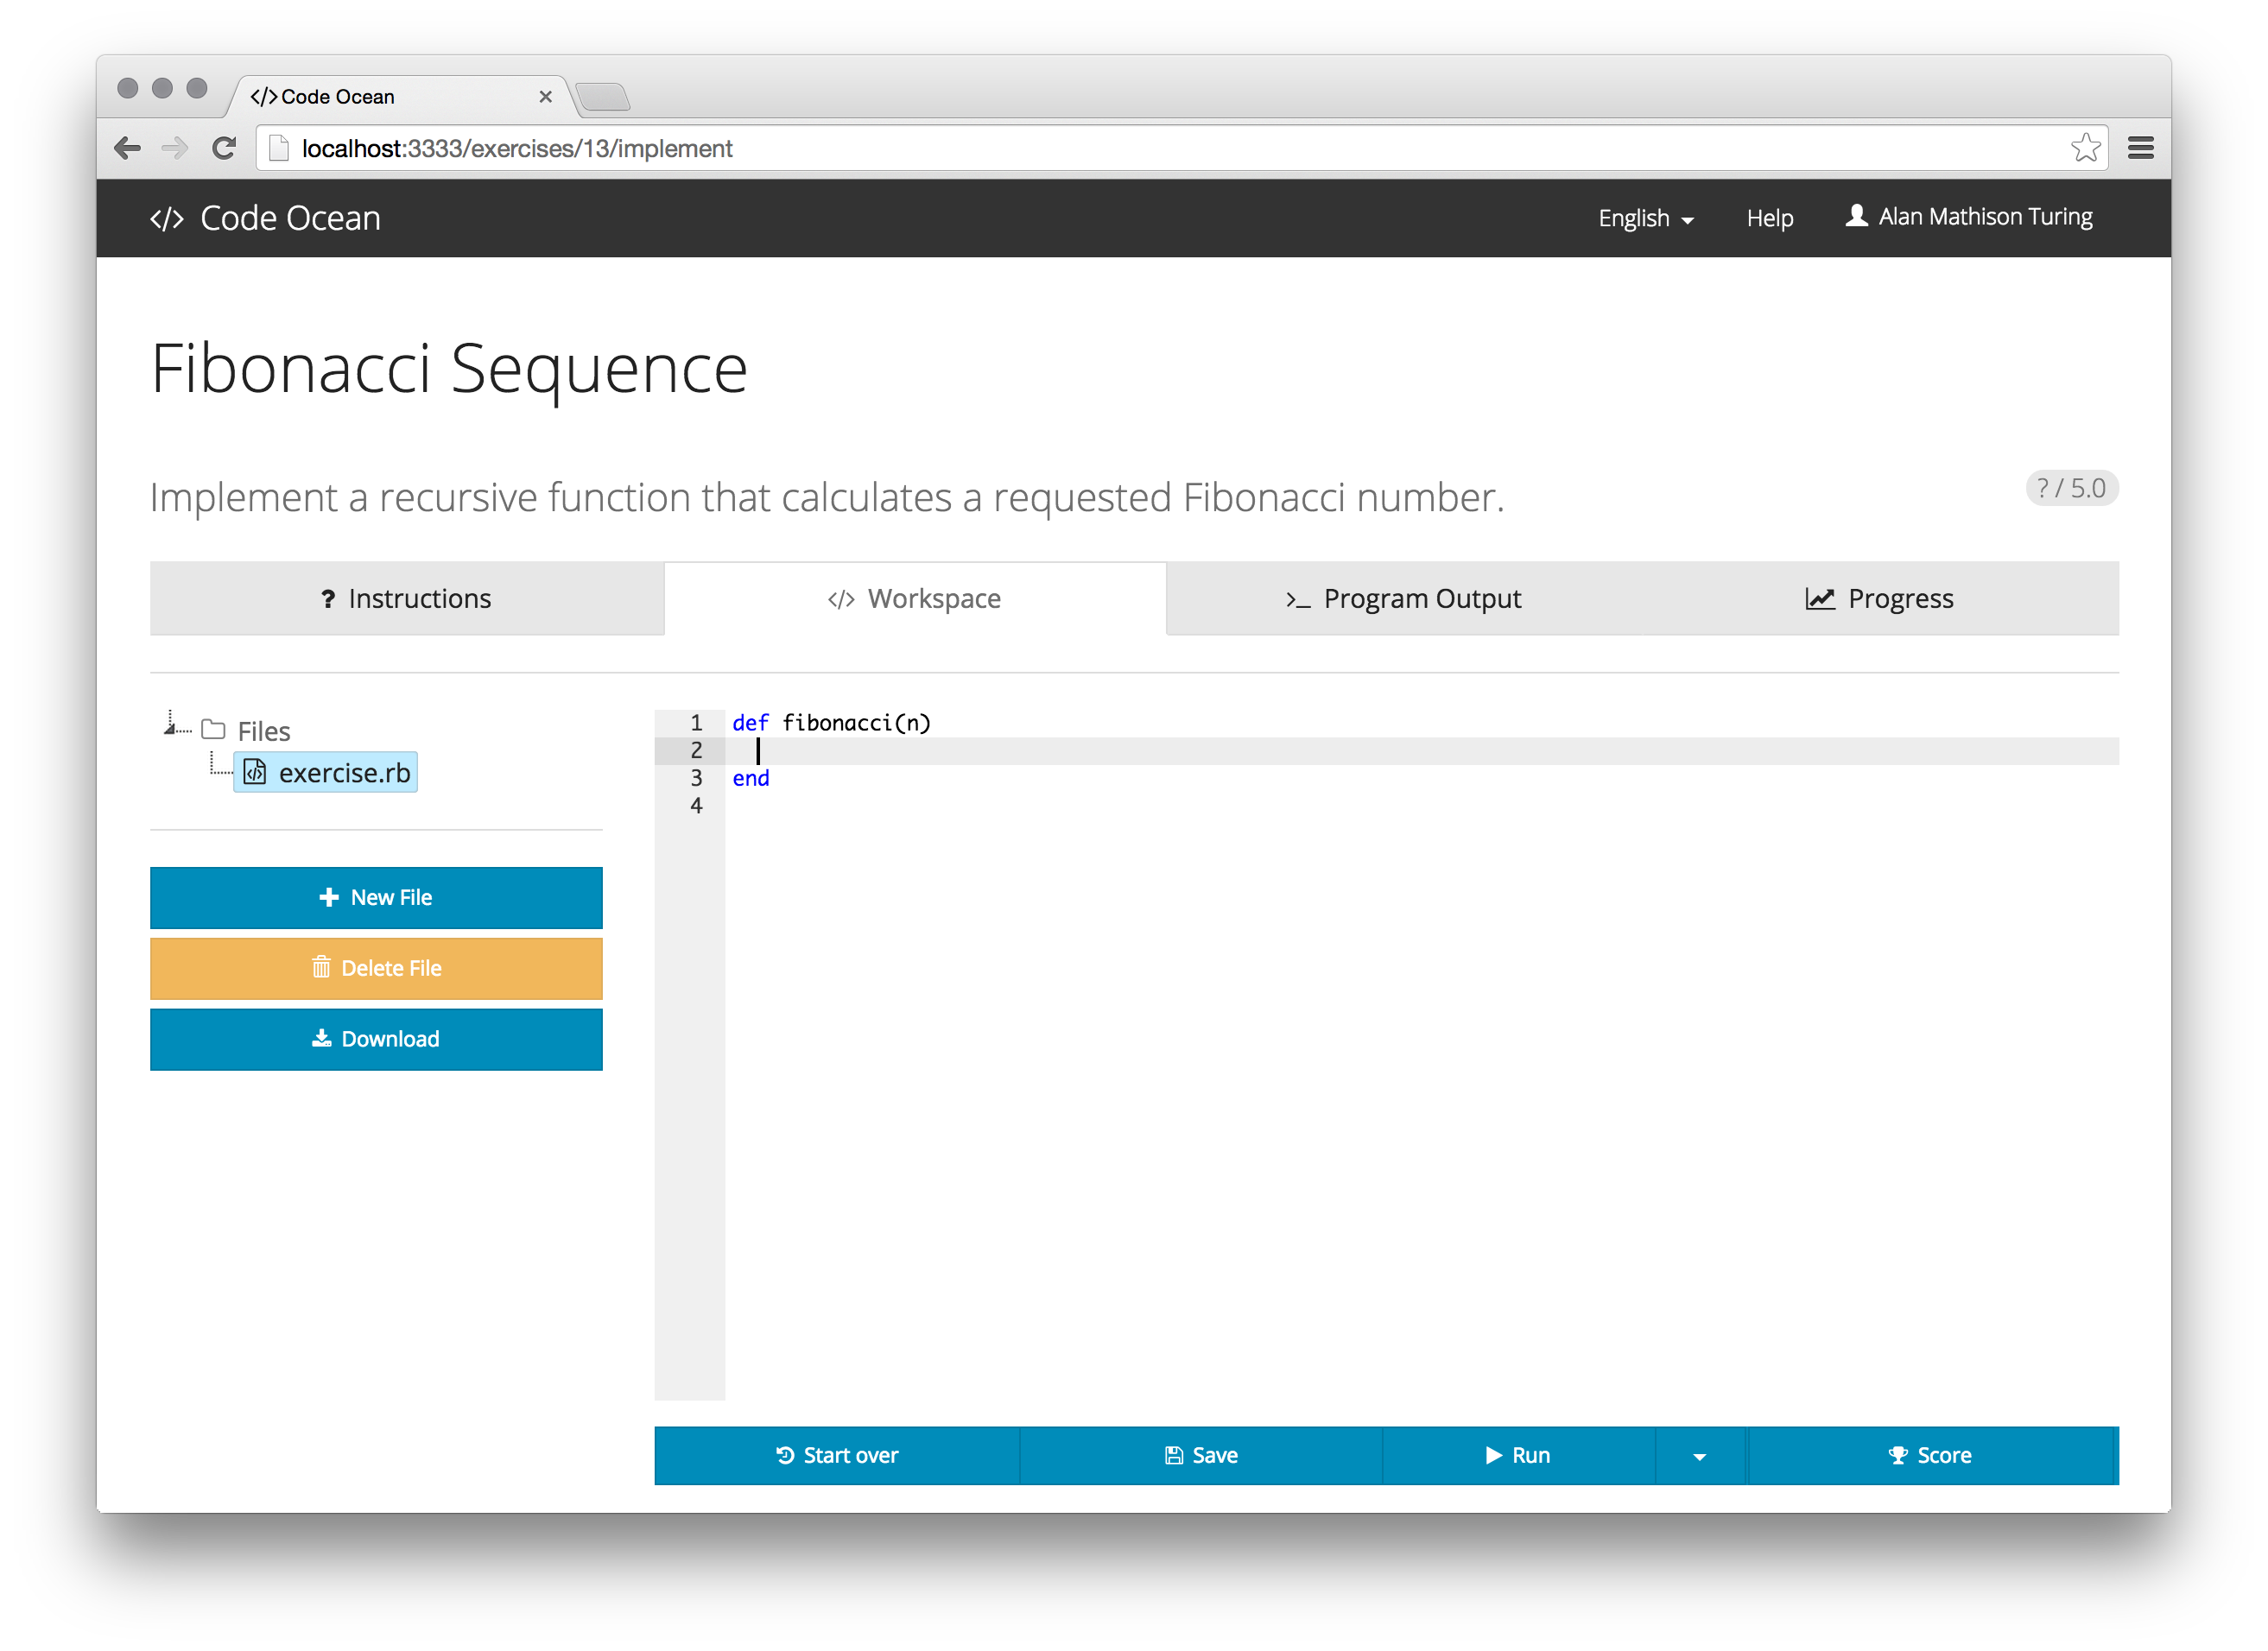
\includegraphics[width=\textwidth]{images/development-environment1.png}
\vspace{-1cm}
\caption{Development Environment: Workspace}
\label{figure:development-environment1}
\end{figure}

\subsection{Composition}

The upper part of the view contains the active exercise's title and description, as well as the most recent score as determined by running the learner's solution against the exercise's tests. The navigation bar at the top of the window allows to control the \gls{ui}'s language and to access help.

Although a certain proficiency in English is usually required in the field of programming~\cite{staubitz2014lightweight}, we decided to facilitate the use of \tool by performing internationalization. While the application is currently available in English and German, further translations can be added with little effort.

The help provided by \tool comprises general directions on how to use the application as well as further information specific to the active exercise's execution environment. These resources are aimed to compensate for the missing face-to-face instructor involvement in the context of \moocs~\cite{pieterse2013automated}.

\begin{figure}
\centering
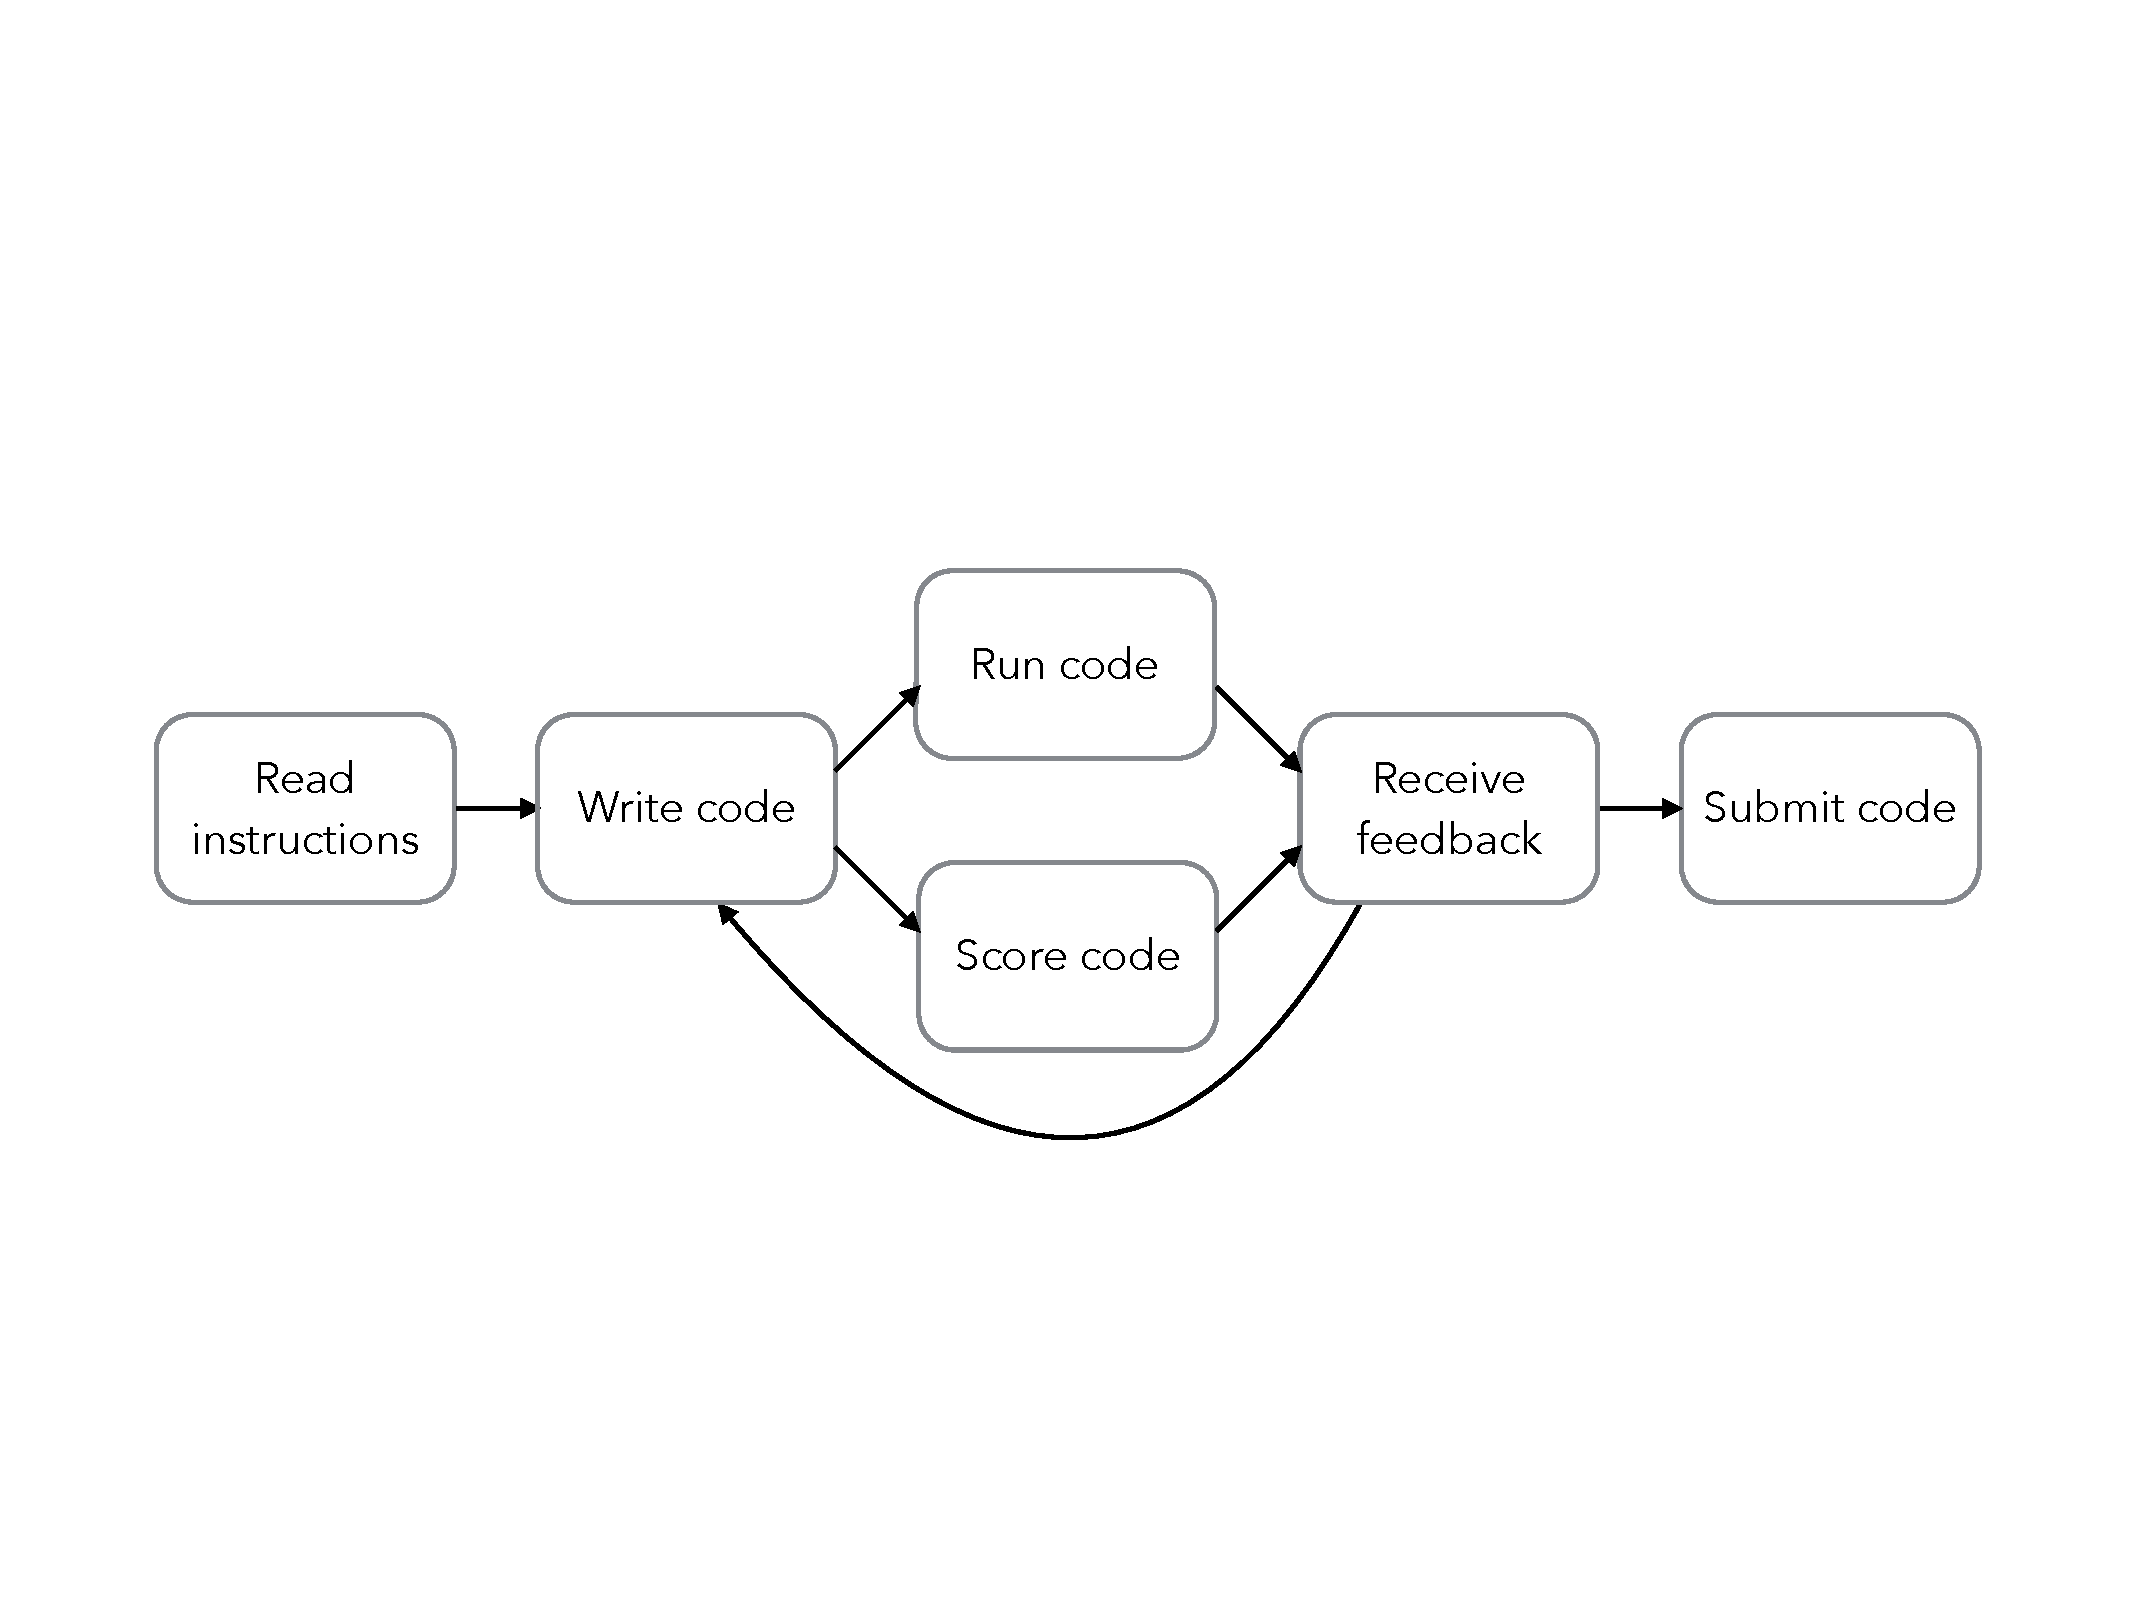
\includegraphics[clip=true, trim=2.5cm 7.7cm 2.5cm 9.6cm, width=\textwidth]{images/development-process}
\caption{Iterative Development Process}
\label{figure:development-process}
\end{figure}

The major part of the development environment is split up into four tabbed areas, each of which is associated to a step in learners' iterative development workflow depicted in Figure~\ref{figure:development-process}. As switching between these tabs is common, they can be accessed using keyboard shortcuts.

\newpage

The four areas are organized as follows:

\begin{itemize}
\item
  The first tab displays the exercise instructions. It is visible in the beginning of a programming session and can be revisited whenever the learner wants to review the specification. Exercise instructions may include the problem description, expected program behavior in edge cases, exemplary code snippets, and more. To enable a clear and visually appealing presentation, instructions are composed and rendered using Markdown\foo{http://daringfireball.net/projects/markdown/}.
\item
  The second tab hosts the development environment's core component, which is the programming workspace. It is described in detail below.
\item
  The third tab presents program output. Depending on the context, it contains output produced during the execution of learner-written code or during the execution of tests for the purpose of assessment. If the output refers to a program error for which a hint has been provided, the corresponding hint message is displayed along with the original output.
\item
  The fourth tab is dedicated to the student's implementation progress. It displays an overview of the most recent test run, including the total score, partial scores, and feedback regarding the submission's deviations from the specification. A button allows to finish implementation and submit the code for final grading.
\end{itemize}

\subsection{Workspace}

The development environment's workspace is composed of a file tree, a code editing area, as well as some controls for development tasks.

\subsubsection{File Tree}

The visible files associated to an exercise are displayed in an interactive file tree, provided by jsTree\foo{http://www.jstree.com/}. In order to construct the file tree, a tree data structure is populated with the exercise's files and is transformed into the \gls{json} representation expected by jsTree.

\begin{listing}
\inputminted[frame=lines]{rb}{listings/file_tree.rb}
\vspace{-0.33cm}
\caption{Excerpt from the \mintinline{rb}{FileTree} Class}
\label{listing:file_tree}
\end{listing}

Listing~\ref{listing:file_tree} depicts an excerpt from the \mintinline{rb}{FileTree} class, which is responsible for the second part of the process. In order to map a populated tree to the expected data format, \mintinline{rb}{to_js_tree} is called, which recursively calls \mintinline{rb}{map_to_js_tree} for every node in the tree, starting at the root node. Depending on the file represented by a tree node, \mintinline{rb}{map_to_js_tree} returns an object describing the node's visual representation, including caption, icon, and child nodes.

Buttons below the file tree allow users to create, delete, and download files. The ability to create custom workspace files enables learners to practice program design and modularization by splitting up their code into functional units of their own choice.

\subsubsection{Editors}

\tool's web-based development environment is based on Ace, an embeddable open-source code editor, written in JavaScript. We chose Ace from the set of available code editors due to its rich functionality, good reputation, and active maintenance. Ace is a popular and established piece of software, used within many web applications, such as Cloud9, Codecadamy, and GitHub, just to mention a few.

Ace offers source code editing capabilities that match the functionality and performance of native desktop editors. Its rich feature set includes syntax highlighting for a myriad of programming languages, \gls{ui} theming, code folding, automatic indent, keyboard shortcuts, find-and-replace functionality, and more. Consequently, Ace offers a powerful foundation for \tool's development environment.

\tool utilizes multiple Ace editors for providing editing capabilities for all non-binary workspace files. At the beginning of a programming session, all editors are populated with their associated files' contents. Syntax highlighting, code indentation, and syntax validation are set up according to the files' types. Whenever a code snapshot has to be created, all editors' contents are obtained and sent to the server.

Binary workspace files are not displayed in editors. Instead, they are integrated in a way that depends on their type. Binary files that can be rendered by web browsers, such as supported audio files, image files, and video files, are directly embedded. Non-renderable binary files are linked.

\subsubsection{Controls}

A button bar underneath the editors provides controls associated to development tasks:

\begin{itemize}
\item
  The first button allows learners to start over from the beginning by rejecting their changes and resetting all files to the version that the teacher has provided.
\item
  The second button serves to save the code. Since code is always implicitly saved before execution, explicit saving is principally useful for pausing a programming session.
\item
  Depending on the selected workspace file, the third button serves the purpose of executing the file, stopping an active execution, or rendering the file on client side. The rendering option only applies to file types that are natively supported by web browsers, such as \gls{gif}, \gls{html}, JavaScript, and \gls{svg}.
\item
  The fourth button triggers assessment of the current implementation.
\end{itemize}

A student can execute her code as often as desired, for instance to explore its behavior, to understand side effects, and to try out edge cases. This explorative mode of programming can be helpful to uncover flaws indicated by a failing test and to identify the necessary corrective actions~\cite{vihavainen2012multi}.

Moreover, learners can also test their code as frequently as desired. Therefore, feedback received from test executions can be used to iteratively solve the exercise.
